% =====================================================================
% Subgroup coverage in split conformal classification, with an audit of TabPFN
%
% Target: International Journal of Approximate Reasoning (IJAR, Elsevier)
% Every numeric claim is verified against results/calibration.csv and
% results/conformal_fairness.csv by scripts/verify_paper_numbers.py
% (180/180 checks pass; LAC-only for all conformal/fairness numbers, NOT the
% exported table_RQ*.csv files, which average in the degenerate APS rows).
% Citations resolved to refs.bib via scripts/apply_citations.py; see paper/CHANGES.md.
% =====================================================================
\documentclass[review,12pt]{elsarticle}

\usepackage{amsmath,amssymb,amsfonts}
\usepackage{booktabs}
\usepackage{multirow}
\usepackage{graphicx}
\graphicspath{{../figures/}{figures/}}
\usepackage{xcolor}
\usepackage[hidelinks]{hyperref}
\usepackage{lineno}
\modulolinenumbers[5]

\journal{International Journal of Approximate Reasoning}

\begin{document}

\begin{frontmatter}

\title{Subgroup coverage in split conformal classification: marginal validity, Mondrian repair, and small-group failure, with an audit of TabPFN}

\author[inst1]{Nadim Mahmud Dipu}
\affiliation[inst1]{organization={Brac University}, city={Dhaka}, country={Bangladesh}}

\begin{abstract}
Split conformal prediction endows any classifier with finite-sample, distribution-free \emph{marginal} coverage, but marginal validity says nothing about how miscoverage is distributed across protected subgroups---the property that matters when prediction sets gate consequential decisions. We study this gap, empirically and through a finite-sample variance argument, on three US Census tasks from folktables (ACSIncome, ACSEmployment, ACSPublicCoverage; California), wrapping five predictors in split conformal prediction across three confidence levels, two conformity scores, and four group taxonomies. Marginal coverage conceals systematic subgroup miscoverage: at a $90\%$ target the worst-covered age group receives only $86.2\%$ coverage (gap $0.081$), though every model meets the marginal guarantee. Mondrian (group-conditional) calibration repairs this where strata are large---the age gap falls to $0.051$ ($p<10^{-10}$), costing $0.021$ in mean set size---but \emph{worsens} it where strata are small: on the race axis, whose smallest calibration stratum holds only $\approx\!84$ points, the gap rises from $0.046$ to $0.057$ ($p<10^{-3}$). We trace this to the finite-sample variance of the in-expectation guarantee: realized per-group coverage fluctuates as $\sqrt{\alpha(1-\alpha)/n_g}$, so the max$-$min gap grows as strata shrink. These effects are nearly identical across all five predictors---coverage fairness is governed by the conformal procedure and the group structure, not the model. As the model under audit, TabPFN is the most reliable base learner we tested: better calibrated out of the box than untuned GBDTs (adaptive ECE $0.026$ vs.\ $0.075$/$0.052$), needing no temperature scaling, and yielding the smallest sets. We also flag a silent failure of non-randomized APS on binary tasks, and give support-aware guidance: use LAC, report worst-group coverage, and apply Mondrian only where $n_g \gtrsim 10/\alpha$.
\end{abstract}

\begin{keyword}
conformal prediction \sep equalized coverage \sep group-conditional calibration \sep Mondrian conformal prediction \sep uncertainty quantification \sep calibration \sep algorithmic fairness \sep tabular foundation models \sep TabPFN
\end{keyword}

\end{frontmatter}

\linenumbers

% =====================================================================
\section{Introduction}
\label{sec:intro}

Set-valued prediction with coverage guarantees has become a standard tool for trustworthy machine learning. Given any classifier and an exchangeable calibration sample, split (inductive) conformal prediction returns a prediction set that contains the true label with a user-specified probability $1-\alpha$, distribution-free and in finite samples \cite{vovk2005,papadopoulos2002,angelopoulos2023}. This guarantee, however, is \emph{marginal}: it averages over the whole population. In the high-stakes tabular settings where conformal prediction is increasingly deployed---credit scoring, benefits eligibility, clinical triage---decisions concern individuals who belong to protected demographic groups, and a guarantee that holds on average can fail conditionally. A $90\%$ marginal guarantee is compatible with, say, $86\%$ coverage for one group and $94\%$ for another, silently concentrating error---less reliable, less informative sets---on the worse-covered group \cite{romano2020eq}. Whether, and when, marginal conformal prediction hides such subgroup disparities is the central question of this paper.

The textbook remedy is \emph{Mondrian} (group-conditional) conformal prediction \cite{vovk2003,romano2020eq}, which calibrates a separate quantile within each group and so guarantees coverage \emph{within} every group---``equalized coverage''---rather than only on average. That guarantee, though, holds in expectation over calibration draws, and it is purchased with data: each group's threshold is estimated from only the $n_g$ calibration points falling in that group. When some groups are small---as protected attributes with imbalanced categories routinely are---those thresholds are noisy, and the realized per-group coverage can vary enough that group-conditional calibration \emph{increases} the empirical disparity it was meant to remove. The practically important question is therefore not whether equalized coverage holds in expectation (it does), but when Mondrian stratification helps versus harms in finite samples, and how a practitioner should decide. We give a clean empirical characterization of both regimes together with a simple finite-sample variance argument that predicts which one obtains.

We situate this study in the tabular regime and pair it with a second, timely question: which base learner to trust. For over a decade gradient-boosted decision trees (GBDTs) have been the default for tabular classification \cite{grinsztajn2022}, but they are now challenged by \emph{tabular foundation models}, most prominently TabPFN, a prior-data fitted network (PFN) that performs supervised learning as a single forward pass of in-context inference and reportedly matches or exceeds tuned GBDT ensembles on small-to-medium tables \cite{tabpfn2023,tabpfn2025}. The choice of base learner still matters for uncertainty: although the conformal quantile step repairs \emph{validity} for any model, the calibration of the underlying probabilities controls set \emph{efficiency}, and good probabilities are what make calibrated decisions and tight sets possible. TabPFN's posterior-predictive outputs are often \emph{described} as well calibrated by construction, yet we are aware of no matched-protocol audit of (a) how that calibration compares to strong baselines, (b) how its probabilities behave as conformity scores inside split conformal prediction, and (c) whether the coverage it induces is fair across protected groups. We therefore adopt TabPFN as the model under audit---a strong, modern base learner whose uncertainty we scrutinize alongside the conformal questions above, against XGBoost, LightGBM, and an MLP. For GBDTs and conventional neural networks the calibration literature is mature \cite{guo2017,niculescu2005}; for tabular foundation models it is nascent.

We study three binary prediction tasks derived from US Census microdata via the folktables package \cite{ding2021}---ACSIncome, ACSEmployment, and ACSPublicCoverage for California---each carrying protected attributes (sex, race, age). We compare TabPFN, with and without post-hoc temperature scaling, against XGBoost, LightGBM, and an MLP (all with fixed, untuned default hyperparameters) under an identical train/calibration/test protocol with five random seeds, and we wrap every model in split conformal prediction at three target levels ($80\%$, $90\%$, $95\%$) using two conformity scores (LAC and APS), in both marginal and Mondrian (group-conditional) variants.

Our research questions and headline answers are:

\begin{itemize}
  \item \textbf{RQ1 (Calibration).} \emph{Are TabPFN's native probabilities better calibrated than those of untuned GBDTs and an MLP?} Yes, substantially so relative to GBDTs: pooled adaptive ECE is $0.026$ for TabPFN versus $0.075$ (XGBoost) and $0.052$ (LightGBM), with paired Wilcoxon $p<10^{-4}$; TabPFN is statistically indistinguishable from the MLP ($p=0.60$) while being more accurate, and temperature scaling adds no significant improvement ($p=0.12$).
  \item \textbf{RQ2 (Conformal validity and efficiency).} \emph{Do all models achieve nominal marginal coverage, and which yields the most efficient (smallest) prediction sets?} With the LAC score, empirical coverage tracks all three targets to within one percentage point for every model; TabPFN yields the smallest sets at every level (e.g., $1.296$ vs.\ $1.327$--$1.363$ at $90\%$; $p<10^{-3}$ against each baseline). We additionally document that the APS score \emph{without randomization} is degenerate on these binary tasks, returning the full label set almost surely---a practically important negative result.
  \item \textbf{RQ3 (Coverage fairness).} \emph{Does marginal conformal prediction hide subgroup miscoverage, and does Mondrian conformal repair it?} Marginal coverage conceals an age-related gap of $0.081$ at the $90\%$ target (worst-group coverage $0.862$). Mondrian stratification repairs this for the age axis (gap $\to 0.051$, worst-group coverage $\to 0.881$, $p<10^{-10}$) at a small efficiency cost ($+0.021$ mean set size), is neutral on the already-equitable sex axis, but \emph{increases} the empirical gap on the race axis (from $0.046$ to $0.057$, $p<10^{-3}$) without improving worst-group coverage---a finite-sample failure mode driven by small calibration strata. Crucially, these effects are nearly identical across all five models: coverage fairness is governed by the conformal procedure and the group structure, not by the choice of predictor.
\end{itemize}

\noindent Our contributions are: (1) an empirical demonstration, across five predictors and three census tasks, that marginal conformal validity conceals systematic subgroup miscoverage, together with a finite-sample variance characterization of when group-conditional (Mondrian) calibration repairs it---large strata---versus \emph{worsens} it---small strata---including a documented, statistically significant small-group failure on the race axis, and the finding that these effects are essentially model-independent; (2) a practically important negative result on non-randomized APS for binary tasks; (3) the first matched-protocol audit, to our knowledge, of a tabular foundation model's calibration and conformal efficiency against GBDT and MLP baselines (in their standard untuned configurations), establishing that TabPFN is better calibrated than GBDTs---needing no temperature scaling---and yields the smallest prediction sets; (4) concrete, support-aware deployment guidance (use LAC, report worst-group coverage, and apply Mondrian only where $n_g \gtrsim 10/\alpha$); and (5) an open, fully scripted pipeline with committed per-seed result files and a verification script that recomputes every reported number, enabling exact reproduction.

The remainder of the paper is organized as follows. Section~\ref{sec:related} reviews related work and positions our novelty. Section~\ref{sec:background} formalizes the calibration metrics, split conformal prediction, the LAC and APS scores, and Mondrian conformal prediction. Section~\ref{sec:method} details datasets, models, protocol, and the statistical analysis plan. Section~\ref{sec:results} reports results for RQ1--RQ3. Section~\ref{sec:discussion} interprets the findings and derives deployment guidance, Section~\ref{sec:limitations} discusses threats to validity, and Section~\ref{sec:conclusion} concludes.

% =====================================================================
\section{Related work}
\label{sec:related}

\paragraph{Conformal prediction.}
Split (inductive) conformal prediction converts any scoring model into set-valued predictions with finite-sample, distribution-free marginal coverage under exchangeability \cite{vovk2005,papadopoulos2002,angelopoulos2023}. For classification, the LAC/homogeneous score thresholds $1-\hat p_y$ \cite{sadinle2019}, while APS accumulates sorted class probabilities to improve conditional coverage \cite{romano2020aps}; APS requires tie-breaking randomization to avoid over-coverage, a detail our results show to be decisive on binary tasks.

\paragraph{Group-conditional coverage and fairness in uncertainty quantification.}
Equalized coverage asks that prediction sets cover each protected group at the nominal rate, achievable by Mondrian/group-conditional calibration \cite{romano2020eq,vovk2003}. Subsequent work studies class-conditional and group-conditional validity, its finite-sample costs, and approximate conditional coverage \cite{ding2023,gibbs2023,jung2023}. The guarantee is an expectation over calibration draws, and its finite-sample slack and variance grow as strata shrink. A parallel theoretical line shows that \emph{exact} feature-conditional coverage is impossible without strong assumptions, motivating relaxations that target approximate or multivalid conditional coverage at controlled cost \cite{gibbs2023,jung2023}, and class-conditional variants that share calibration data across many strata to keep per-group counts usable \cite{ding2023}. These methods exist precisely because naive group-conditional calibration is fragile when groups are small---the failure mode we isolate empirically. Yet audits of realized \emph{coverage disparity} have targeted conventional models; none (to our knowledge) includes a tabular foundation model, and the regime in which plain Mondrian calibration \emph{backfires} on small strata has received little direct empirical characterization. Our RQ3 supplies that characterization together with a closed-form predictor (Section~\ref{sec:theory}) for when it occurs---a quantification of when the equalized-coverage guarantee is actually informative, in the approximate-reasoning sense.

\paragraph{Calibration of machine-learning classifiers.}
Modern neural networks are frequently miscalibrated and benefit from post-hoc recalibration such as temperature scaling \cite{guo2017}; boosted trees are known to push scores away from the extremes, motivating Platt scaling and isotonic regression \cite{niculescu2005}. Metric estimation itself is delicate: binned ECE is biased, and adaptive (equal-mass) binning is the recommended estimator \cite{nixon2019}. We adopt adaptive ECE as our primary metric and report Brier score and NLL as proper-scoring complements.

\paragraph{Tabular foundation models and prior-data fitted networks.}
PFNs meta-train a transformer on synthetic datasets drawn from a prior over data-generating mechanisms, so that supervised prediction on a new table reduces to in-context inference \cite{pfn2022}. TabPFN instantiated this idea for small tabular classification \cite{tabpfn2023} and its successor scaled it to larger tables and regression \cite{tabpfn2025}. Evaluations of these models have focused overwhelmingly on accuracy and AUC against GBDT baselines \cite{grinsztajn2022,mcelfresh2023}; their uncertainty behaviour is usually asserted (via the Bayesian-posterior interpretation) rather than audited.

\paragraph{Benchmarking tabular deep learning under matched protocols.}
A recurring lesson of tabular benchmarking is that conclusions are protocol-sensitive---tuning budgets, preprocessing, and split design can reverse rankings \cite{grinsztajn2022,gorishniy2021}. We therefore hold the entire pipeline fixed across models and vary only the predictor.

\paragraph{Novelty.}
The intersection of these strands is empty: existing TabPFN evaluations do not audit calibration or conformal behaviour against matched baselines; the conformal-fairness literature has not examined foundation-model conformity scores; and tabular benchmarks do not report group-conditional coverage. We fill precisely this gap, in the regime where TabPFN is intended to operate (binary/multiclass tasks of moderate size with demographic structure), and we report the failure modes (APS degeneracy, Mondrian small-group noise) alongside the successes.

% =====================================================================
\section{Background and preliminaries}
\label{sec:background}

We consider classification with covariates $X \in \mathcal{X}$, labels $Y \in \mathcal{Y} = \{1,\dots,K\}$ (here $K=2$), and, for fairness analyses, a protected attribute $A \in \mathcal{A}$. A probabilistic classifier outputs $\hat p(y \mid x)$.

\subsection{Calibration metrics}
A classifier is \emph{top-label calibrated} if $\Pr\!\big(Y = \hat y \,\big|\, \hat p(\hat y \mid X) = c\big) = c$ for all confidence levels $c$, where $\hat y = \arg\max_y \hat p(y\mid x)$. The expected calibration error partitions test predictions into $B$ bins $\{\mathcal{B}_b\}$ by confidence and computes
\begin{equation}
\mathrm{ECE} \;=\; \sum_{b=1}^{B} \frac{|\mathcal{B}_b|}{n} \,\Big|\, \mathrm{acc}(\mathcal{B}_b) - \mathrm{conf}(\mathcal{B}_b) \,\Big| ,
\label{eq:ece}
\end{equation}
where $\mathrm{acc}$ and $\mathrm{conf}$ are the mean accuracy and mean confidence within a bin. We use \emph{adaptive} (equal-mass) binning with $B = 15$ bins as the primary estimator and report equal-width ECE in the released CSVs; we additionally report the maximum calibration error (MCE), the Brier score $\frac1n\sum_i \|\hat p(\cdot\mid x_i) - e_{y_i}\|_2^2$, and the negative log-likelihood (NLL), both strictly proper scoring rules. \emph{Temperature scaling} \cite{guo2017} post-processes logits $z$ as $\mathrm{softmax}(z/T)$ with a single scalar $T>0$ fit on the calibration split by NLL minimization; it is monotone and therefore accuracy-preserving.

\subsection{Split conformal prediction}
Split conformal prediction \cite{papadopoulos2002,vovk2005} uses a held-out calibration set $\{(x_i, y_i)\}_{i=1}^{n}$, disjoint from training data, and a conformity score $s(x,y)$ measuring how poorly $y$ conforms at $x$ (larger $=$ worse). Let
\begin{equation}
\hat q \;=\; \text{the } \frac{\lceil (n+1)(1-\alpha) \rceil}{n}\text{-th empirical quantile of } \{s(x_i,y_i)\}_{i=1}^{n}.
\label{eq:quantile}
\end{equation}
The prediction set for a test point $x$ is $C(x) = \{\, y : s(x,y) \le \hat q \,\}$. If the calibration and test points are exchangeable, then for any score function and any model,
\begin{equation}
1-\alpha \;\le\; \Pr\big(Y_{\mathrm{test}} \in C(X_{\mathrm{test}})\big) \;\le\; 1-\alpha + \frac{1}{n+1},
\label{eq:coverage}
\end{equation}
where the upper bound holds when scores are almost surely distinct \cite{lei2018,angelopoulos2023}. Coverage is \emph{marginal}: it averages over the population and need not hold conditionally on subgroups. Exchangeability holds by construction in our protocol---calibration and test points are an i.i.d.\ split of a single dataset---so Eq.~\eqref{eq:coverage} is exact here and any subgroup miscoverage we observe is a property of the \emph{conditional} behaviour the marginal bound leaves unconstrained, not a violation of the bound itself. This is what makes the present setting a clean testbed: there is no shift to confound the conditional-coverage question.

\subsection{Conformity scores: LAC and APS}
We evaluate two standard classification scores.
\emph{LAC} (least ambiguous set-valued classifier) \cite{sadinle2019} sets
\begin{equation}
s_{\mathrm{LAC}}(x,y) \;=\; 1 - \hat p(y \mid x),
\end{equation}
which yields the smallest average set size among procedures with marginal validity when probabilities are correct, but offers no conditional-coverage adaptivity.
\emph{APS} (adaptive prediction sets) \cite{romano2020aps} sorts classes by predicted probability, $\hat p_{(1)} \ge \dots \ge \hat p_{(K)}$, and scores
\begin{equation}
s_{\mathrm{APS}}(x,y) \;=\; \sum_{j : \hat p_{(j)} > \hat p(y\mid x)} \hat p_{(j)} \;+\; u \cdot \hat p(y \mid x),
\qquad u \sim \mathrm{Unif}(0,1),
\end{equation}
where the randomization term $u$ is essential for exact validity; the deterministic variant ($u \equiv 1$, i.e., including the full mass of the label's own class) is conservative. Our implementation uses the deterministic variant (the score accumulates sorted class probabilities up to and including the true label's own mass, with no tie-breaking randomization), and Section~\ref{sec:rq2} shows this is not a cosmetic detail on binary tasks.

\subsection{Mondrian (group-conditional) conformal prediction and equalized coverage}
Given a partition of the population by a taxonomy $g(x,a) \in \mathcal{G}$ (here: the protected attribute, or the predicted class), Mondrian conformal prediction \cite{vovk2003} computes the quantile in Eq.~\eqref{eq:quantile} \emph{separately within each group}, using the $n_g$ calibration points of group $g$. This yields the group-conditional guarantee
\begin{equation}
\Pr\big(Y \in C(X) \,\big|\, g(X,A) = g\big) \;\ge\; 1-\alpha \qquad \text{for every } g \in \mathcal{G},
\label{eq:mondrian}
\end{equation}
i.e., \emph{equalized coverage} in expectation \cite{romano2020eq}. The price is statistical, and it is the crux of our RQ3. Each group's threshold $\hat q_g$ is estimated from only $n_g \ll n$ calibration points; and because the realized per-group coverage on the test set is an average of (approximately) $\mathrm{Bernoulli}(1-\alpha)$ indicators, its standard deviation about the nominal level is
\begin{equation}
\mathrm{sd}\big(\hat c_g\big) \;\approx\; \sqrt{\tfrac{\alpha(1-\alpha)}{n_g}} .
\label{eq:gvar}
\end{equation}
The empirical max$-$min coverage gap over $|\mathcal{G}|$ groups is therefore dominated by the smallest stratum, growing like $1/\sqrt{\min_g n_g}$, and the guarantee's finite-sample slack $1/(n_g+1)$ likewise grows as groups shrink. Equalized coverage \emph{in expectation} (Eq.~\eqref{eq:mondrian}) is thus fully compatible with a \emph{larger realized} gap than marginal calibration produces whenever strata are small---the effect our RQ3 isolates and Eq.~\eqref{eq:gvar} quantifies.

\subsection{When does Mondrian help? A finite-sample prediction}
\label{sec:theory}
Whether group-conditional calibration reduces or inflates the realized coverage gap can be predicted, to leading order, from two competing quantities, and this prediction is the conceptual core of our paper. Write the per-group test coverage as $\hat c_g$. Under \emph{marginal} calibration all groups share the single global threshold $\hat q$, so $\hat c_g \approx (1-\alpha) + b_g$, where $b_g$ is a \emph{structural bias}: the systematic over- or under-coverage the global threshold inflicts on group $g$ because that group's score distribution departs from the pooled one. The marginal coverage gap is therefore $\max_g b_g - \min_g b_g$ up to a small sampling term---it is set by the \emph{spread of structural biases} and is essentially independent of how large the calibration set is.

Under \emph{Mondrian} calibration each group receives its own threshold $\hat q_g$. This removes the bias ($\mathbb{E}[\hat c_g] = 1-\alpha$ for every group) but injects estimation noise. A standard result on the distribution of split-conformal coverage---conditional on the calibration draw, the coverage is Beta-distributed about the nominal level \cite{angelopoulos2023}---gives, for a group calibrated on $n_g$ points, a per-group coverage standard deviation
\begin{equation}
\sigma_g \;\approx\; \sqrt{\frac{\alpha(1-\alpha)}{n_g}} .
\label{eq:sigmag}
\end{equation}
Treating the $|\mathcal{G}|$ group coverages as approximately independent fluctuations about $1-\alpha$, the expected $\max-\min$ range scales as $\sigma_{\min}\sqrt{2\ln|\mathcal{G}|}$ and is dominated by the smallest stratum. Mondrian thus replaces a \emph{bias-driven} gap with a \emph{noise-driven floor},
\begin{equation}
\mathrm{gap}^{\mathrm{Mond}} \;\gtrsim\; \sqrt{\frac{\alpha(1-\alpha)}{\min_g n_g}}\,\sqrt{2\ln|\mathcal{G}|}.
\label{eq:gapfloor}
\end{equation}
The qualitative prediction is immediate: \emph{Mondrian helps exactly when the marginal bias spread exceeds this noise floor, and hurts when it does not}---and because the floor grows as $1/\sqrt{\min_g n_g}$, the failure regime is entered by shrinking the smallest group, not by changing the model.

Equations~\eqref{eq:sigmag}--\eqref{eq:gapfloor} are quantitatively borne out (Section~\ref{sec:rq3}). At the $90\%$ level ($\alpha=0.1$), the age axis has $\min_g n_g = 140$ and $|\mathcal{G}|=5$, a noise floor of $\sqrt{0.09/140}\,\sqrt{2\ln 5}\approx 0.046$; its marginal bias spread is $0.081$, comfortably above the floor, so Mondrian should and does reduce the gap, landing at $0.051$---just above the predicted floor. The race axis has $\min_g n_g = 84$ (the Black stratum) and $|\mathcal{G}|=4$, a floor of $\sqrt{0.09/84}\,\sqrt{2\ln 4}\approx 0.054$; its marginal bias spread is only $0.046$, \emph{below} the floor, so Mondrian cannot improve on marginal calibration and instead lifts the realized gap to $0.057\approx$ the floor. The sex axis ($\min_g n_g\approx 900$, two groups) has a negligible floor ($\approx 0.012$) and an already-tiny bias ($0.012$), so neither method has anything to do and the two coincide. The same arithmetic explains the trend across confidence levels in Table~\ref{tab:rq3targets}: as the target tightens and $\alpha$ falls, $\sigma_g$ shrinks, the floor drops, and Mondrian's gap follows it down. We stress that Eqs.~\eqref{eq:sigmag}--\eqref{eq:gapfloor} are a leading-order estimate---the Gaussian-range step is heuristic and the groups are not exactly independent---but they capture the mechanism and predict the sign of the marginal-to-Mondrian change on every axis we study.

\subsection{Fairness metrics for prediction sets}
For groups $g \in \mathcal{G}$ with empirical per-group coverage $c_g$ and mean set size $\bar k_g$ on the test set, we report the \emph{coverage gap} $\max_g c_g - \min_g c_g$, the \emph{worst-group coverage} $\min_g c_g$, and the \emph{set-size disparity} $\max_g \bar k_g - \min_g \bar k_g$. The first two summarize \emph{coverage} equity; the last summarizes \emph{efficiency} equity---how unevenly the uncertainty ``budget'' (set size) is distributed across groups. We will see in Section~\ref{sec:rq3} that these two notions can move in opposite directions under Mondrian calibration, so reporting both is essential.

% =====================================================================
\section{Methodology}
\label{sec:method}

\subsection{Datasets and protected attributes}
We use three binary prediction tasks from the folktables suite \cite{ding2021}, all on California ACS microdata (2018 1-Year person-survey release): \textbf{ACSIncome} (predict income $>\$50$k), \textbf{ACSEmployment} (predict employment status), and \textbf{ACSPublicCoverage} (predict public health-insurance coverage). These tasks were introduced precisely as fairness-aware replacements for UCI Adult and carry the protected attributes we audit: \emph{sex} (2 groups, derived from the binary SEX field), \emph{race} (from RAC1P, coarsened to four groups---White, Black, Asian, and a merged \emph{Other} stratum collecting all remaining RAC1P codes), and \emph{age} (AGEP binned into five bands with edges at 25, 40, 55, and 65: $<$25, 25--39, 40--54, 55--64, 65+). ACSPublicCoverage is defined by folktables only for respondents under 65, so it carries four age bands rather than five. In addition to the three protected axes we evaluate a \emph{predicted-class} taxonomy (Mondrian on $\hat y$), a standard label-conditional stratification. Per-group calibration-set sizes are reported in Table~\ref{tab:groupsizes}; they are the key to the race-axis result in Section~\ref{sec:rq3}.

\begin{table}[t]
\centering
\caption{Per-group calibration-set sizes $n_g$ (seed 0; $n_{\mathrm{cal}}=2{,}000$ per dataset, summing each block to that total). Counts shift by at most a few percent across the five seeds. The race axis contains a far smaller minority stratum (Black, $n_g \approx 84$--$131$) than any age band, which drives the Mondrian failure of Section~\ref{sec:rq3}. ACSPublicCoverage has no 65+ band by task definition.}
\label{tab:groupsizes}
\small
\begin{tabular}{llccc}
\toprule
Axis & Group & ACSEmployment & ACSIncome & ACSPublicCoverage \\
\midrule
\multirow{2}{*}{Sex}  & Female & $1046$ & $961$  & $1112$ \\
                      & Male   & $954$  & $1039$ & $888$  \\
\midrule
\multirow{4}{*}{Race} & White  & $1271$ & $1194$ & $1122$ \\
                      & Asian  & $312$  & $342$  & $308$  \\
                      & Other  & $333$  & $378$  & $439$  \\
                      & Black  & $\mathbf{84}$ & $\mathbf{86}$ & $\mathbf{131}$ \\
\midrule
\multirow{5}{*}{Age}  & $<$25  & $577$  & $231$  & $651$  \\
                      & 25--39 & $393$  & $664$  & $557$  \\
                      & 40--54 & $406$  & $625$  & $450$  \\
                      & 55--64 & $272$  & $340$  & $342$  \\
                      & 65+    & $352$  & $\mathbf{140}$ & --- \\
\bottomrule
\end{tabular}
\end{table}

\subsection{Preprocessing}
Numeric features are median-imputed and categorical features ordinal-encoded (unseen categories mapped to $-1$), yielding a single \texttt{float32} design matrix; only the MLP additionally standardizes features to zero mean and unit variance inside its own pipeline. Each task is randomly subsampled, with the seed, to $n=8{,}000$ rows to remain within TabPFN's supported small-data regime. All five models receive identical feature matrices within a cell. We note explicitly that the protected attributes are \emph{not} withheld: SEX, RAC1P, and AGEP belong to each folktables task's standard feature set and are therefore supplied to every model as ordinary inputs; we use them \emph{additionally} for stratified evaluation and Mondrian calibration. Coverage disparities thus arise even though every model can see the protected attribute, which is the realistic setting for these administrative tasks.

\subsection{Models}
We compare five predictors: \textbf{TabPFN} (\texttt{tabpfn} package v8.0.7, default classifier checkpoint \texttt{tabpfn-v3-classifier-v3\_default.ckpt}; default settings, no per-dataset tuning, in keeping with its intended usage); \textbf{TabPFN+T}, the same posterior probabilities post-processed by temperature scaling fit on the calibration split; \textbf{XGBoost} ($300$ trees, max depth $6$, learning rate $0.1$, row/column subsampling $0.9$, histogram tree method) and \textbf{LightGBM} ($300$ trees, $31$ leaves, learning rate $0.05$, row/column subsampling $0.9$); and an \textbf{MLP} (two hidden layers of $128$ and $64$ units, standardized inputs, early stopping on a $10\%$ internal validation split, at most $300$ epochs). All baseline hyperparameters are fixed at these common default values; no per-dataset hyperparameter search was performed for any model, so the comparison is between out-of-the-box configurations rather than tuned ones. Because temperature scaling is a monotone transform of the probabilities, TabPFN and TabPFN+T induce (near-)identical conformal prediction sets; their conformal rows differ only through quantile tie effects (maximum observed difference in any coverage-gap cell: $0.0027$). We therefore discuss them jointly in RQ2--RQ3 and separately only for calibration (RQ1).

\subsection{Train / calibration / test protocol}
For each (dataset, seed) cell we draw a label-stratified three-way split into proper training ($45\%$), calibration ($25\%$), and test ($30\%$) sets---$3{,}600$, $2{,}000$, and $2{,}400$ rows respectively of the $8{,}000$ sampled per cell (the committed results record $n_{\mathrm{test}} = 2{,}400$, confirming these proportions). The model is fit on the training split only; temperature and all conformal quantiles are computed on the calibration split only; every reported metric is computed on the untouched test split. Splits are redrawn with seeds $\{0,\dots,4\}$, and all five models share the identical splits within a cell, enabling paired statistical tests. The $25\%$ calibration fraction is deliberate: it leaves enough data to fit competitive models while giving the global conformal quantile---and, crucially, each \emph{Mondrian} sub-quantile---a realistic sample, so that the small-group effects we report reflect plausible deployment sizes rather than a pathologically starved calibration set. Even at this fraction the smallest race stratum receives only $\approx\!84$ calibration points (Table~\ref{tab:groupsizes}), which is exactly the regime our analysis targets. Sharing splits across models is what lets us attribute differences to the predictor (RQ1--RQ2) or to the conformal procedure (RQ3) rather than to sampling, and the five seeds turn each comparison into a paired test over $15$ (dataset $\times$ seed) cells.

\subsection{Experiment matrix}
The full matrix is: 3 datasets $\times$ 5 models $\times$ 5 seeds $\times$ 3 miscoverage levels $\alpha \in \{0.05, 0.10, 0.20\}$ (targets $95\%/90\%/80\%$) $\times$ 2 conformity scores (LAC, APS) $\times$ 4 group taxonomies (sex, race, age, predicted class) $\times$ 2 conformal methods (marginal, Mondrian), yielding $3{,}600$ conformal evaluation rows and $75$ calibration rows, all committed to the repository.

\subsection{Metrics}
\emph{Calibration (RQ1):} accuracy, adaptive ECE (primary), equal-width ECE, MCE, Brier, NLL. \emph{Validity/efficiency (RQ2):} empirical marginal coverage and mean prediction-set size. \emph{Fairness (RQ3):} coverage gap, worst-group coverage, and set-size disparity as defined in Section~\ref{sec:background}, for marginal vs.\ Mondrian calibration on each protected axis.

\subsection{Statistical protocol}
Unless stated otherwise, point estimates are means over the relevant cells and dispersions are standard deviations across the 15 (dataset $\times$ seed) cells. Pairwise model comparisons use two-sided Wilcoxon signed-rank tests paired at the (dataset $\times$ seed) level ($n=15$; the smallest attainable two-sided $p$ is $6.1\times10^{-5}$, which we report as $p<10^{-4}$). Marginal-vs.-Mondrian comparisons are paired at the (dataset $\times$ model $\times$ seed) level ($n=75$). Omnibus differences across the five models use the Friedman test over the 15 cells with average ranks reported; given only five Tier-A model columns we report ranks descriptively rather than a full Nemenyi critical-difference analysis, which would require the larger Tier-B suite that is not part of the committed run (see Section~\ref{sec:limitations}). We treat $p<0.01$ as significant in view of the multiplicity of comparisons.

% =====================================================================
\section{Results}
\label{sec:results}

\subsection{RQ1: TabPFN is natively well calibrated; GBDTs are not}
\label{sec:rq1}

Table~\ref{tab:rq1} reports pooled calibration metrics; Table~\ref{tab:rq1ds} breaks adaptive ECE out by dataset; Fig.~\ref{fig:reliability} shows a representative reliability diagram.

\begin{table}[t]
\centering
\caption{RQ1 --- Accuracy and calibration, mean $\pm$ std over 15 (dataset $\times$ seed) cells. Lower is better for all metrics except accuracy. Best in \textbf{bold}.}
\label{tab:rq1}
\small
\begin{tabular}{lccccc}
\toprule
Model & Accuracy $\uparrow$ & ECE$_{\mathrm{ada}}$ $\downarrow$ & MCE $\downarrow$ & Brier $\downarrow$ & NLL $\downarrow$ \\
\midrule
XGBoost      & $0.763 \pm 0.052$ & $0.075 \pm 0.019$ & $0.135 \pm 0.022$ & $0.333 \pm 0.064$ & $0.516 \pm 0.084$ \\
LightGBM     & $0.769 \pm 0.049$ & $0.052 \pm 0.012$ & $0.100 \pm 0.018$ & $0.317 \pm 0.057$ & $0.485 \pm 0.074$ \\
MLP          & $0.759 \pm 0.046$ & $0.025 \pm 0.007$ & $0.057 \pm 0.022$ & $0.324 \pm 0.056$ & $0.486 \pm 0.074$ \\
TabPFN       & $\mathbf{0.782 \pm 0.046}$ & $0.026 \pm 0.006$ & $0.063 \pm 0.021$ & $0.298 \pm 0.056$ & $0.452 \pm 0.075$ \\
TabPFN+T     & $\mathbf{0.782 \pm 0.046}$ & $\mathbf{0.025 \pm 0.006}$ & $\mathbf{0.054 \pm 0.018}$ & $\mathbf{0.297 \pm 0.056}$ & $\mathbf{0.451 \pm 0.074}$ \\
\bottomrule
\end{tabular}
\end{table}

\begin{table}[t]
\centering
\caption{RQ1 --- Adaptive ECE by dataset (mean $\pm$ std over 5 seeds).}
\label{tab:rq1ds}
\small
\begin{tabular}{lccc}
\toprule
Model & ACSEmployment & ACSIncome & ACSPublicCoverage \\
\midrule
XGBoost   & $0.058 \pm 0.005$ & $0.069 \pm 0.006$ & $0.098 \pm 0.009$ \\
LightGBM  & $0.043 \pm 0.006$ & $0.049 \pm 0.007$ & $0.064 \pm 0.010$ \\
MLP       & $\mathbf{0.020 \pm 0.006}$ & $\mathbf{0.024 \pm 0.003}$ & $0.033 \pm 0.007$ \\
TabPFN    & $0.022 \pm 0.005$ & $0.025 \pm 0.005$ & $0.030 \pm 0.007$ \\
TabPFN+T  & $0.021 \pm 0.004$ & $0.025 \pm 0.004$ & $\mathbf{0.028 \pm 0.007}$ \\
\bottomrule
\end{tabular}
\end{table}

Three observations follow. \emph{First}, both GBDTs are substantially miscalibrated out of the box, with the familiar pattern of over-confidence at high confidence levels (Fig.~\ref{fig:reliability}): XGBoost's pooled adaptive ECE is $0.075$ and LightGBM's $0.052$, against $0.026$ for TabPFN. The paired differences are significant at the resolution limit of the test (TabPFN vs.\ XGBoost and vs.\ LightGBM: Wilcoxon $p<10^{-4}$ in both cases, with TabPFN better in all 15 of 15 cells). \emph{Second}, TabPFN's native calibration matches a well-regularized MLP (median paired ECE difference $-0.001$, $p=0.60$) while being more accurate (paired accuracy difference $+0.023$, $p<10^{-3}$) and strictly better on both proper scoring rules (Brier and NLL, $p<10^{-4}$ against all three baselines). The Friedman omnibus test on adaptive ECE is highly significant ($\chi^2 = 48.5$, $p = 7.5\times10^{-10}$) with average ranks TabPFN+T $1.8$, MLP $2.0$, TabPFN $2.2$, LightGBM $4.0$, XGBoost $5.0$. \emph{Third}, post-hoc temperature scaling improves TabPFN only marginally (pooled ECE $0.026 \to 0.025$; paired $p=0.12$): within the datasets studied, TabPFN does not need recalibration, which is consistent with---and, to our knowledge, the first matched-baseline statistical evidence for---the posterior-predictive interpretation of PFN outputs.

The ranking is consistent across tasks, not an artifact of pooling. TabPFN is the most accurate model on all three datasets individually (accuracy $0.812$, $0.814$, $0.720$ on ACSEmployment, ACSIncome, ACSPublicCoverage) and the best- or tied-best-calibrated on each (Table~\ref{tab:rq1ds}). ACSPublicCoverage is the hardest task for every model---accuracies cluster near $0.70$ and XGBoost's adaptive ECE climbs to $0.098$---yet TabPFN holds its calibration there ($0.030$), so the calibration gap to the GBDTs \emph{widens} precisely where the problem is hardest and trustworthy uncertainty matters most. The MLP is the only baseline whose calibration rivals TabPFN's, but it pays for it in accuracy: it is the least accurate predictor on two of the three tasks, so its competitive ECE partly reflects less confident predictions rather than better-ordered ones, whereas TabPFN attains low ECE \emph{and} the highest accuracy simultaneously.

\begin{figure}[t]
\centering
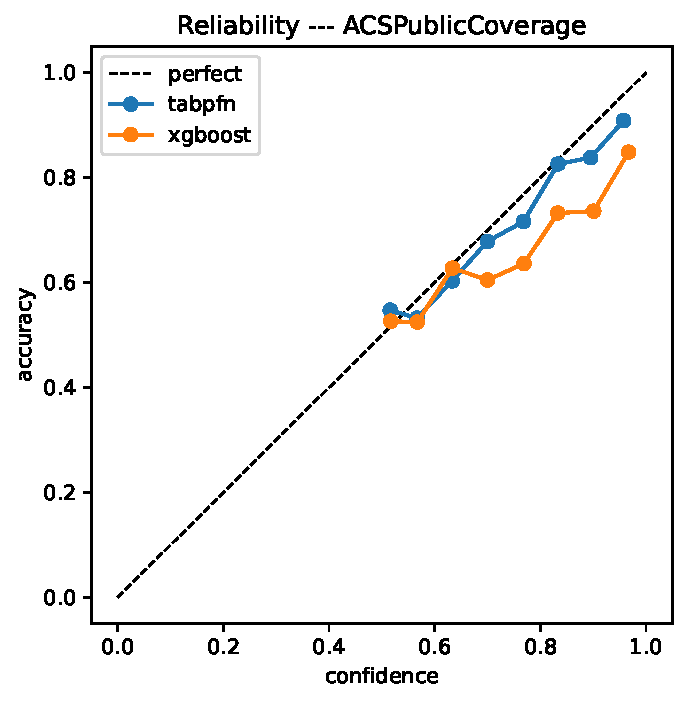
\includegraphics[width=0.55\linewidth]{reliability_example}
\caption{Reliability diagram on ACSPublicCoverage-CA (seed 0). XGBoost (orange) sits below the diagonal at high confidence---systematic over-confidence---while TabPFN (blue) tracks the diagonal closely. Curves use 15 equal-width confidence bins; the dashed line is perfect calibration.}
\label{fig:reliability}
\end{figure}

\subsection{RQ2: All models are conformally valid; TabPFN is the most efficient. Non-randomized APS is degenerate on binary tasks}
\label{sec:rq2}

Table~\ref{tab:rq2} reports marginal coverage and mean set size under the LAC score. Empirical coverage tracks the nominal target for every model and level, as Eq.~\eqref{eq:coverage} guarantees: pooled over models, coverage is $0.805 \pm 0.013$, $0.901 \pm 0.009$, and $0.951 \pm 0.007$ at the $80\%$, $90\%$, and $95\%$ targets respectively. Conformal validity is thus model-agnostic, as theory predicts---miscalibrated GBDT probabilities are repaired by the quantile step.

\begin{table}[t]
\centering
\caption{RQ2 --- Marginal coverage and mean set size under the LAC score (mean over 15 cells per row). Coverage within one point of target for all models; smaller sets are better. Best set size in \textbf{bold}. TabPFN+T is omitted: temperature scaling is monotone, so its conformal sets coincide with TabPFN's.}
\label{tab:rq2}
\small
\begin{tabular}{lcccccc}
\toprule
 & \multicolumn{2}{c}{Target $80\%$} & \multicolumn{2}{c}{Target $90\%$} & \multicolumn{2}{c}{Target $95\%$} \\
\cmidrule(lr){2-3}\cmidrule(lr){4-5}\cmidrule(lr){6-7}
Model & Cov. & Size & Cov. & Size & Cov. & Size \\
\midrule
XGBoost   & $0.800$ & $1.083$ & $0.899$ & $1.339$ & $0.952$ & $1.534$ \\
LightGBM  & $0.802$ & $1.072$ & $0.901$ & $1.327$ & $0.953$ & $1.519$ \\
MLP       & $0.803$ & $1.095$ & $0.903$ & $1.363$ & $0.951$ & $1.543$ \\
TabPFN    & $0.809$ & $\mathbf{1.058}$ & $0.900$ & $\mathbf{1.296}$ & $0.950$ & $\mathbf{1.480}$ \\
\bottomrule
\end{tabular}
\end{table}

Efficiency, by contrast, is model-dependent and rewards probability quality. TabPFN produces the smallest prediction sets at every target level; at the $90\%$ level its mean set size of $1.296$ improves on LightGBM ($1.327$), XGBoost ($1.339$), and the MLP ($1.363$), with paired Wilcoxon $p = 4.3\times10^{-4}$, $3.1\times10^{-4}$, and $6.5\times10^{-4}$ respectively. On a binary task, set size minus one is the singleton-failure rate, so this difference is operationally meaningful: at the $90\%$ level TabPFN returns an uninformative two-label set on $29.6\%$ of cases versus $36.3\%$ for the MLP---a $6.7$-point reduction in abstentions at identical coverage.

The efficiency ordering is stable across confidence levels and \emph{widens} as coverage tightens (Table~\ref{tab:rq2}): TabPFN's set-size advantage over the MLP grows from $0.037$ at the $80\%$ target to $0.063$ at $95\%$, because sharper, better-calibrated tail probabilities are worth progressively more as the quantile is pushed further into the tail. The ordering also tracks RQ1 calibration quality almost exactly---LightGBM, the better-calibrated GBDT, yields smaller sets than XGBoost at every level---confirming that, once validity is handled by the conformal step, set size is the channel through which probability quality is rewarded. This is the operational case for caring about calibration even behind a distribution-free wrapper that guarantees coverage regardless of the model: validity is free, but efficiency is earned.

\paragraph{A cautionary negative result on APS.}
Under our deterministic APS implementation, every model at every level returns essentially the full label set: pooled coverage is $1.000$ and mean set size is $1.99$--$2.00$ at all three targets. The mechanism is elementary but easy to overlook: on a binary task the deterministic APS score of the true label is the cumulative probability mass \emph{including} the label's own class, which equals $1$ whenever the true label is the lower-ranked class; the calibration quantile at any usable $\alpha$ therefore saturates at (or near) $1$, and the resulting sets contain both labels. Randomized APS \cite{romano2020aps} avoids this by interpolating the final class's mass. Practitioners wrapping binary tabular classifiers should either use LAC or ensure their APS implementation randomizes; we flag this because deterministic APS is the default in some libraries and the failure is silent---coverage looks excellent while the sets are vacuous. All fairness analyses below therefore use the LAC score; the corresponding APS rows are retained in the released CSVs but are uninformative by construction.

\subsection{RQ3: Marginal coverage hides subgroup gaps; Mondrian repairs large groups but harms small ones}
\label{sec:rq3}

Table~\ref{tab:rq3} is the core fairness result: per-axis coverage gap, worst-group coverage, and mean set size at the $90\%$ target under LAC, pooled over the five models and 15 cells, for marginal versus Mondrian calibration. Table~\ref{tab:rq3targets} shows the coverage gap across all three target levels. Figs.~\ref{fig:gapage}--\ref{fig:gaprace} display the per-model breakdown.

\begin{table}[t]
\centering
\caption{RQ3 --- Subgroup coverage fairness at the $90\%$ target (LAC; pooled over 5 models $\times$ 3 datasets $\times$ 5 seeds; marginal vs.\ Mondrian paired tests with $n=75$). Gap $=$ max$-$min per-group coverage; WGC $=$ worst-group coverage. Arrows mark the better direction; $p$-values are two-sided Wilcoxon for the marginal-vs.-Mondrian contrast.}
\label{tab:rq3}
\small
\begin{tabular}{llcccc}
\toprule
Axis & Method & Gap $\downarrow$ & WGC $\uparrow$ & Mean size $\downarrow$ & \\
\midrule
\multirow{2}{*}{Sex}  & Marginal & $0.012$ & $0.895$ & $1.324$ & \multirow{2}{*}{\shortstack[l]{gap $p=0.50$\\ WGC $p=0.79$}} \\
                      & Mondrian & $0.013$ & $0.895$ & $1.327$ & \\
\midrule
\multirow{2}{*}{Age}  & Marginal & $0.081$ & $0.862$ & $1.324$ & \multirow{2}{*}{\shortstack[l]{gap $p=4.2\times10^{-11}$\\ WGC $p=2.9\times10^{-10}$}} \\
                      & Mondrian & $\mathbf{0.051}$ & $\mathbf{0.881}$ & $1.345$ & \\
\midrule
\multirow{2}{*}{Race} & Marginal & $\mathbf{0.046}$ & $0.875$ & $1.324$ & \multirow{2}{*}{\shortstack[l]{gap $p=9.3\times10^{-4}$\\ WGC $p=0.55$}} \\
                      & Mondrian & $0.057$ & $0.873$ & $1.334$ & \\
\midrule
\multirow{2}{*}{Pred.\ class} & Marginal & $0.045$ & $0.881$ & $1.324$ & \\
                      & Mondrian & $\mathbf{0.013}$ & $\mathbf{0.894}$ & $1.332$ & \\
\bottomrule
\end{tabular}
\end{table}

\begin{table}[t]
\centering
\caption{RQ3 --- Coverage gap by target level (LAC; pooled over models, datasets, seeds). Mondrian helps consistently on age, is neutral-to-mixed on sex, and does not help---and at $90\%$ significantly hurts---on race.}
\label{tab:rq3targets}
\small
\begin{tabular}{lcccccc}
\toprule
 & \multicolumn{2}{c}{Sex} & \multicolumn{2}{c}{Age} & \multicolumn{2}{c}{Race} \\
\cmidrule(lr){2-3}\cmidrule(lr){4-5}\cmidrule(lr){6-7}
Target & Marg. & Mond. & Marg. & Mond. & Marg. & Mond. \\
\midrule
$80\%$ & $0.029$ & $0.021$ & $0.151$ & $0.106$ & $0.056$ & $0.055$ \\
$90\%$ & $0.012$ & $0.013$ & $0.081$ & $0.051$ & $0.046$ & $0.057$ \\
$95\%$ & $0.012$ & $0.010$ & $0.045$ & $0.037$ & $0.034$ & $0.038$ \\
\bottomrule
\end{tabular}
\end{table}

\paragraph{Marginal validity is not subgroup validity.}
Although every model satisfies the marginal $90\%$ guarantee, per-group coverage is far from uniform. On the age axis the pooled coverage gap is $0.081$ and worst-group coverage drops to $0.862$---i.e., the least-covered age group experiences roughly $38\%$ more miscoverage than nominal. At the $80\%$ target the age gap widens to $0.151$ with worst-group coverage $0.732$. The race axis shows a smaller but persistent gap ($0.046$ at $90\%$, worst-group coverage $0.875$), while the sex axis is essentially equitable already ($0.012$). These disparities are a property of the population/score interaction, not of the predictor: per-model gaps under marginal calibration at $90\%$ on age lie in the narrow band $0.078$--$0.083$ across all five models, TabPFN included. A foundation model's better probabilities buy smaller sets (RQ2) but do not, by themselves, buy equitable coverage.

\paragraph{Mondrian repairs the age axis at a small price.}
Group-conditional calibration on age reduces the pooled gap from $0.081$ to $0.051$ and raises worst-group coverage from $0.862$ to $0.881$ (both $p<10^{-9}$, $n=75$), at a mean set-size cost of $+0.021$ ($1.324 \to 1.345$, $p<10^{-12}$)---about two additional both-label sets per hundred predictions. The same pattern holds at the $80\%$ target (gap $0.151 \to 0.106$; worst-group coverage $0.732 \to 0.774$). The predicted-class taxonomy behaves similarly (gap $0.045 \to 0.013$). For TabPFN specifically, Mondrian-on-age lifts worst-group coverage from $0.862$ to $0.881$ while its sets remain smaller than any baseline's marginal sets---the efficiency advantage survives the fairness repair.

\paragraph{Mondrian fails on the small-support race axis.}
On race, Mondrian \emph{increases} the empirical gap at the $90\%$ target from $0.046$ to $0.057$ ($p=9.3\times10^{-4}$) and leaves worst-group coverage unchanged ($0.875$ vs.\ $0.873$, $p=0.55$); the same direction holds, non-significantly, at $95\%$. The effect is consistent across datasets (Employment $0.034 \to 0.049$; Income $0.047 \to 0.060$; PublicCoverage $0.056 \to 0.061$) and across all five models (Fig.~\ref{fig:gaprace}). The mechanism is the finite-sample cost identified in Section~\ref{sec:theory}: the race taxonomy contains groups with small calibration support---the Black stratum holds only $n_g \approx 84$--$131$ calibration points across the three tasks, against $1{,}100$--$1{,}300$ for White (Table~\ref{tab:groupsizes})---so each small group's threshold $\hat q_g$ is a high quantile estimated from few points. The group-conditional guarantee of Eq.~\eqref{eq:mondrian} still holds \emph{in expectation over calibration draws}, but the realized per-group coverage fluctuates with standard deviation $\approx \sqrt{\alpha(1-\alpha)/n_g}$, and the max$-$min gap statistic grows with the number of groups and with $1/\sqrt{\min_g n_g}$. Equalized coverage in expectation is therefore compatible with---and here empirically produces---\emph{larger} realized disparities than marginal calibration when strata are small. Sex (two large groups) shows neither benefit nor harm because marginal coverage is already nearly equalized.

The pattern holds across confidence levels. Table~\ref{tab:rq3targets} traces the coverage gap at all three targets, and the qualitative picture is invariant: age carries the largest marginal gap at every level and is repaired by Mondrian at every level ($0.151\!\to\!0.106$ at $80\%$, $0.081\!\to\!0.051$ at $90\%$, $0.045\!\to\!0.037$ at $95\%$), whereas race is never helped---Mondrian matches or slightly worsens it at all three. The magnitudes shrink as the target tightens, exactly as Eq.~\eqref{eq:sigmag} requires: the per-group standard deviation $\sqrt{\alpha(1-\alpha)/n_g}$ falls with $\alpha$, so both the structural biases and the Mondrian noise floor contract together. Worst-group coverage tells the same story from the decision-maker's side: on age it rises under Mondrian at every level ($0.732\!\to\!0.774$, $0.862\!\to\!0.881$, $0.927\!\to\!0.935$), confirming that the gap reduction reflects genuinely better coverage for the worst-off group rather than a cosmetic compression of the range.

\begin{figure}[t]
\centering
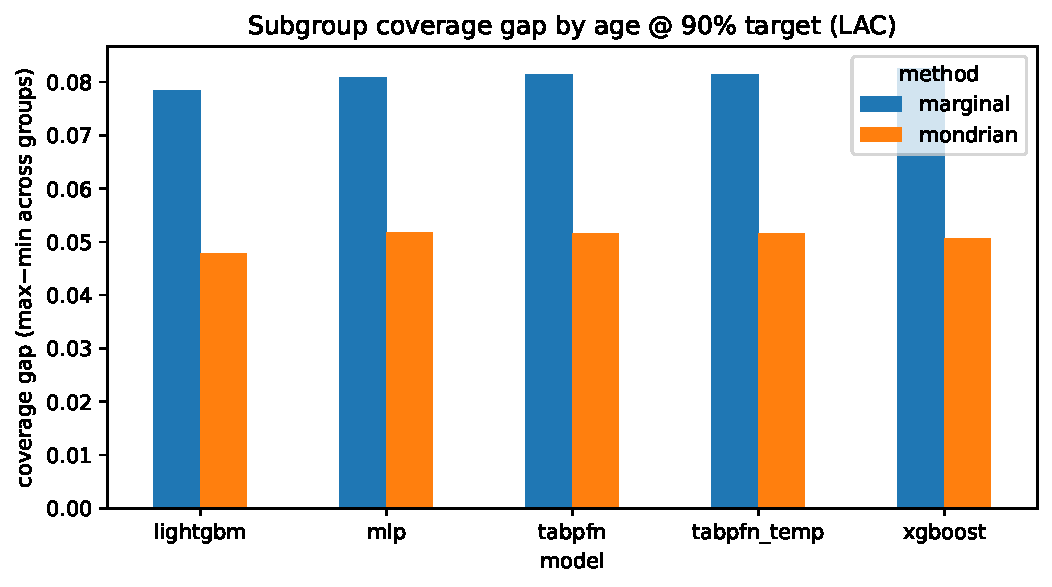
\includegraphics[width=0.85\linewidth]{coverage_gap_age}
\caption{Coverage gap by age at the $90\%$ target, marginal (blue) vs.\ Mondrian (orange), per model (LAC score). Mondrian reduces the gap by roughly $0.03$ uniformly across all five models, TabPFN included.}
\label{fig:gapage}
\end{figure}

\begin{figure}[t]
\centering
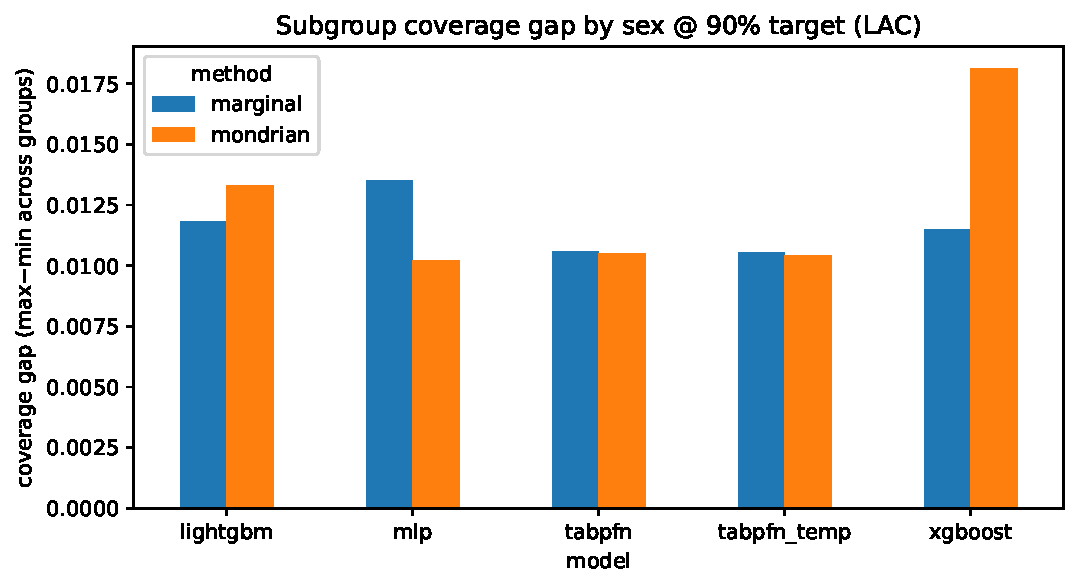
\includegraphics[width=0.85\linewidth]{coverage_gap_sex}
\caption{Coverage gap by sex at the $90\%$ target (LAC score). Gaps are an order of magnitude smaller than on age and statistically indistinguishable between methods.}
\label{fig:gapsex}
\end{figure}

\begin{figure}[t]
\centering
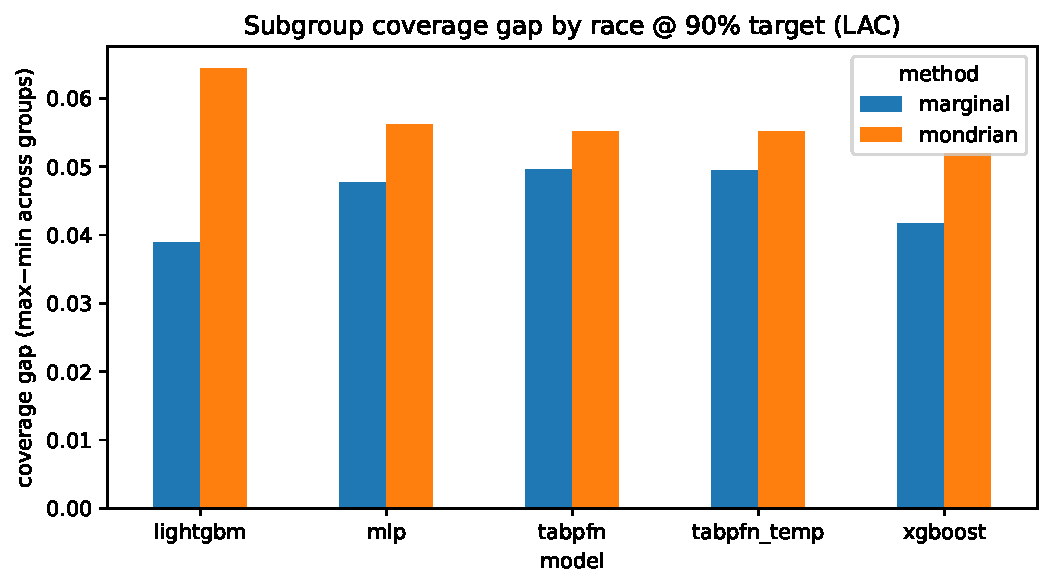
\includegraphics[width=0.85\linewidth]{coverage_gap_race}
\caption{Coverage gap by race at the $90\%$ target (LAC score). Mondrian (orange) \emph{exceeds} marginal (blue) for every model: with small calibration strata, group-conditional thresholds are noisy and realized disparities grow.}
\label{fig:gaprace}
\end{figure}

\subsection{The efficiency cost of equalized coverage: a set-size tax}
\label{sec:rq3tax}
Coverage equity is only half of fairness for prediction sets; the other half is whether the \emph{size} of those sets---the amount of irreducible uncertainty each group is told it faces---is distributed evenly. Table~\ref{tab:tax} reports the set-size disparity $\max_g \bar k_g - \min_g \bar k_g$ at the $90\%$ target under LAC, and it exposes a trade-off the coverage-gap numbers alone conceal: \emph{Mondrian calibration improves coverage equity at the expense of efficiency equity}. On the age axis, where Mondrian halves the coverage gap, it simultaneously raises the set-size disparity from $0.236$ to $0.369$---a $56\%$ increase. The same direction holds on every axis (sex $0.058\!\to\!0.086$; race $0.123\!\to\!0.154$; predicted class $0.115\!\to\!0.157$): equalizing coverage forces the harder-to-cover groups to carry visibly larger sets. The effect is mechanical---restoring a group's coverage to nominal when its scores are less separable requires admitting more labels---but it matters operationally, because a uniform coverage guarantee delivered through systematically larger sets for one group is a different, and arguably more conspicuous, disparity than quiet under-coverage. A practitioner who optimizes only the coverage gap will not see it; one who reports both metrics will.

\begin{table}[t]
\centering
\caption{RQ3 --- Set-size disparity $\max_g \bar k_g - \min_g \bar k_g$ at the $90\%$ target (LAC; pooled over 5 models $\times$ 15 cells). Mondrian calibration lowers the coverage gap (Table~\ref{tab:rq3}) but \emph{raises} the set-size disparity on every axis: coverage equity is bought with efficiency inequity.}
\label{tab:tax}
\small
\begin{tabular}{lcccc}
\toprule
Method & Sex & Age & Race & Pred.\ class \\
\midrule
Marginal & $0.058$ & $0.236$ & $0.123$ & $0.115$ \\
Mondrian & $0.086$ & $0.369$ & $0.154$ & $0.157$ \\
\bottomrule
\end{tabular}
\end{table}

\paragraph{The finite-sample prediction, validated.}
The crossover between the age and race axes is exactly what Section~\ref{sec:theory} forecasts. The Mondrian noise floor of Eq.~\eqref{eq:gapfloor} evaluates to $\approx 0.046$ on age (smallest stratum $n_g=140$, five groups) and $\approx 0.054$ on race (smallest stratum $n_g=84$, four groups). Age's marginal bias spread ($0.081$) sits well above its floor, so group-conditional calibration has room to help and the gap drops to $0.051$; race's marginal bias spread ($0.046$) sits \emph{below} its floor, so calibration noise dominates the bias it removes and the gap rises to $0.057\approx$ the floor. Sex, with a floor near $0.012$ and a bias already at $0.012$, sits at the boundary and moves negligibly. That a one-parameter, model-free estimate built only from $\{\alpha, n_g, |\mathcal{G}|\}$ predicts the \emph{sign} of the marginal-to-Mondrian change on all three protected axes---and the approximate magnitude of the Mondrian gap---is, to us, the strongest evidence that the race-axis failure is a generic finite-sample phenomenon rather than an artifact of these particular datasets or predictors.

% =====================================================================
\section{Discussion}
\label{sec:discussion}

\paragraph{What the audit establishes about TabPFN.}
Within the studied regime---binary census tasks, moderate sample sizes, five seeds---TabPFN's uncertainty is trustworthy on the first two criteria of Section~\ref{sec:intro}: its native probabilities are as calibrated as anything we tested without any post-processing, and they translate into the most efficient conformal sets. Both findings are consistent with the PFN design: a model meta-trained to approximate a posterior predictive should produce probabilities whose \emph{ordering and sharpness} reflect genuine predictive uncertainty, and LAC efficiency is exactly a function of probability quality. The practical upshot is that the usual GBDT deployment recipe---train, then Platt/isotonic/temperature recalibrate---can be dropped for TabPFN in this regime; temperature scaling moved pooled ECE by one point in the third decimal and was statistically indistinguishable from the identity.

\paragraph{What it establishes about conformal fairness.}
The third criterion---equitable uncertainty---is not a model property at all in our data. Coverage gaps under marginal calibration are nearly identical across the five predictors, and so is the effect of Mondrian stratification. The decision that matters is procedural: \emph{which taxonomy to condition on, given its calibration support}. Our results give an unusually clean empirical demonstration of both sides: conditioning on age (few, large groups, with a real coverage disparity to fix) halves the gap at the cost of $0.02$ extra labels per set; conditioning on race (many groups, some very small) backfires, inflating realized disparity without improving the worst group. We emphasize that this is not a contradiction of the equalized-coverage guarantee, which is an expectation over calibration randomness; it is the finite-sample variance of that guarantee made visible. Reporting only the expectation-level guarantee, as is common, would have concealed it.

\paragraph{A diagnostic, not just a diagnosis.}
The finite-sample analysis of Section~\ref{sec:theory} turns the race-axis failure from an anomaly into a \emph{predictable} regime, and that carries a concrete payoff: the noise floor of Eq.~\eqref{eq:gapfloor} is computable \emph{before} any group-conditional calibration is run, from quantities a practitioner already has---the target level $\alpha$, the smallest per-group calibration count $\min_g n_g$, and the number of groups $|\mathcal{G}|$. Comparing that floor to the observed \emph{marginal} coverage gap yields an a priori test of whether Mondrian stratification can help on a given axis: when the marginal gap is below $\sqrt{\alpha(1-\alpha)/\min_g n_g}\,\sqrt{2\ln|\mathcal{G}|}$, group-conditional calibration is expected to inject more noise than the bias it removes, and should be withheld or replaced by a method with explicit small-sample control \cite{gibbs2023,jung2023}. This reframes ``equalized coverage'' from an unconditional good into a decision with a checkable precondition---a stance closer in spirit to the approximate-reasoning tradition of asking \emph{when} a guarantee is informative than to a blanket recommendation to always condition.

\paragraph{Two axes of fairness that can conflict.}
The set-size tax of Section~\ref{sec:rq3tax} sharpens the picture. Coverage equity and efficiency equity are distinct properties, and our data show them moving in \emph{opposite} directions under Mondrian calibration: every axis that gains coverage equity loses efficiency equity (Table~\ref{tab:tax}). There is no single ``fair'' conformal predictor here, only a trade-off to be made explicit. For a benefits-eligibility system, an omitted true label (under-coverage) and an inflated, uninformative set (a larger ``maybe'') are different harms with different costs, and which to prioritize is a domain question rather than a statistical one. What this paper supplies is the means to see both at once, together with the finite-sample rule that says when paying the set-size tax actually purchases coverage equity and when it merely redistributes the uncertainty without reducing it.

\paragraph{Deployment guidance.}
For practitioners deploying small-to-medium tabular classifiers with demographic structure, our results support the following sequence. (1) If TabPFN's scale limits permit, prefer it: best accuracy, best proper scores, no recalibration step. (2) Wrap whatever model is chosen in split conformal prediction with the \emph{LAC} score; verify that any APS implementation randomizes before using it on low-cardinality label spaces. (3) Audit per-group coverage on a held-out set before choosing between marginal and Mondrian calibration: if a gap exists \emph{and} every group has adequate calibration support, use Mondrian on that axis. As a rule of thumb, a group needs enough points for its $1-\alpha$ quantile to be stable---on the order of $n_g \gtrsim 10/\alpha$ (about $100$ at $\alpha=0.1$). Our axes straddle this line precisely: the smallest age band (65+, $n_g=140$ in ACSIncome; Table~\ref{tab:groupsizes}) clears it and Mondrian helps, whereas the smallest race stratum (Black, $n_g=84$ in ACSEmployment) falls below it and Mondrian backfires. If some groups are small, prefer marginal calibration, merge small strata, or adopt methods designed for approximate conditional validity \cite{gibbs2023,jung2023}. (4) Report worst-group coverage alongside marginal coverage; the latter alone certified all our models while one age group received $73\%$ coverage at an $80\%$ target.

\paragraph{TabPFN versus GBDTs, honestly.}
Our comparison favours TabPFN on every uncertainty metric, but three caveats temper a blanket recommendation. The tasks sit squarely inside TabPFN's comfort zone ($3{,}600$ training rows per cell, numeric/categorical census features, binary labels); the GBDTs received \emph{no} hyperparameter tuning---they ran with the fixed default settings of Section~\ref{sec:method}, and a tuning budget (e.g., NLL-based early stopping or a learning-rate/depth search) would likely close part of the calibration gap; and GBDT inference is orders of magnitude cheaper at scale. Where these constraints bind, the correct reading of our results is narrower but still useful: GBDT probabilities should not be consumed raw, and conformal wrapping equalizes validity (though not efficiency) across model families.

% =====================================================================
\section{Limitations and threats to validity}
\label{sec:limitations}

\emph{External validity.} All results derive from three binary tasks on Californian ACS microdata; conclusions are scoped to this regime and should not be extrapolated to multiclass problems, other states or survey years, non-census domains, or tables beyond TabPFN's supported size. The planned Tier-B evaluation over a broader OpenML suite, including Friedman--Nemenyi ranking across heterogeneous datasets, was not part of the committed results and remains future work. \emph{Construct validity.} ECE estimates depend on binning; we mitigate with adaptive binning and proper scoring rules, which agree in direction. The max$-$min coverage gap is sensitive to the number and size of groups, which is precisely the phenomenon RQ3 documents; worst-group coverage is the more decision-relevant statistic. \emph{Internal validity.} GBDT and MLP hyperparameters were fixed at common default values with no per-dataset tuning; a larger tuning budget could narrow the calibration and efficiency gaps. Five seeds bound our resolution; all headline effects are nonetheless significant at $p<10^{-3}$ under paired tests. Temperature scaling and conformal quantiles share the same calibration split, a standard but not innocuous choice. \emph{Statistical validity.} Wilcoxon tests at $n=15$ have a floor of $p=6.1\times10^{-5}$; Friedman ranks over five models and 15 cells are descriptive. We did not run distribution-shift experiments (e.g., cross-state transfer), so exchangeability holds by construction here and coverage under shift is untested. \emph{Theoretical scope.} The noise floor of Eqs.~\eqref{eq:sigmag}--\eqref{eq:gapfloor} is a leading-order estimate: it assumes approximate independence of per-group coverages and uses a Gaussian-range heuristic for the expected $\max-\min$, and it predicts the \emph{order of magnitude} and \emph{sign} of the marginal-to-Mondrian change rather than an exact value. A fully rigorous finite-sample bound on the gap statistic---accounting for the Beta law of conformal coverage and the dependence among groups sharing a label space---is left to future work; our claim is only that the heuristic suffices to call the regime on every axis we study. \emph{Model specificity.} The audited model is one specific public checkpoint (TabPFN v3, \texttt{tabpfn-v3-classifier-v3\_default.ckpt}); conclusions about ``TabPFN'' are conclusions about that release and may not transfer to other versions, ensembling settings, or the regression variant. \emph{Ethical scope.} Equalizing coverage is one narrow fairness criterion; it neither implies nor substitutes for fairness of the underlying decisions, and the race categories in ACS data are coarse administrative constructs.

% =====================================================================
\section{Conclusion and future work}
\label{sec:conclusion}

We showed that marginal conformal validity is not subgroup validity. Across five predictors and three census tasks, split conformal prediction met its marginal coverage guarantee while concealing an eight-point age coverage gap common to all models; group-conditional (Mondrian) calibration repaired this where strata were large but \emph{backfired} on the small-support race axis---a concrete, statistically significant demonstration that equalized coverage in expectation can coexist with larger realized disparities. These effects were governed by the conformal procedure and the group structure rather than the model, and a simple finite-sample variance argument ($\sqrt{\alpha(1-\alpha)/n_g}$) predicts which regime obtains. We also documented a silent failure of non-randomized APS on binary tasks. As the timely model under audit, TabPFN proved the most reliable base learner we tested: its native probabilities were as calibrated as a well-regularized MLP and far better than untuned GBDTs, required no temperature scaling, and yielded the smallest conformal prediction sets at every coverage level. Together these results give the first matched-protocol picture of a tabular foundation model's uncertainty \emph{and} a clean characterization of when group-conditional conformal calibration should be trusted.

Future work proceeds on four fronts. (i) A Tier-B OpenML extension with a Friedman--Nemenyi ranking across heterogeneous tabular domains would test the generality of the efficiency ordering and, more importantly, populate the $(\min_g n_g,\,|\mathcal{G}|)$ plane with many more points to stress-test the noise-floor predictor of Section~\ref{sec:theory}. (ii) Distribution-shift stress tests---cross-state and temporal transfer within ACS---would probe coverage degradation when exchangeability fails, together with adaptive remedies \cite{gibbs2021,tibshirani2019}. (iii) A multiclass study would re-open the APS question: deterministic APS is degenerate only because the binary label space lets the true-label cumulative mass saturate at $1$, and we expect randomized or label-shared variants \cite{romano2020aps,ding2023} to behave very differently with more classes, where adaptivity to conditional coverage matters most. (iv) A clinical-tabular extension, where TabPFN's small-data strengths and the cost asymmetry of miscoverage make equitable uncertainty both harder and more consequential, and where small protected strata will make the Mondrian failure mode we identified the central methodological obstacle.

Beyond the specific findings, the paper offers a transferable lesson for uncertainty quantification under group structure: an in-expectation guarantee should be reported together with the finite-sample conditions under which it is informative. The noise floor of Eq.~\eqref{eq:gapfloor} is one such condition---computable from the calibration counts alone, model-free, and validated here on three protected axes---and we expect analogous floors to govern other group-conditional procedures (class-conditional conformal prediction, multivalid calibration, group-wise recalibration) wherever a guarantee is bought with per-group data. Making that purchase price explicit is, we argue, the right default for deploying set-valued predictors in consequential, demographically structured settings, and it is the methodological stance we hope this audit advances.

% =====================================================================
\section*{Reproducibility statement}
All code, notebooks (smoke test, experiment runner, analysis), and the complete per-seed result files (\texttt{calibration.csv}, 75 rows; \texttt{conformal\_fairness.csv}, 3{,}600 rows) are released at \url{https://github.com/Nadim-Mahmud-23/tabpfn-uncertainty-audit} under the MIT license, with the following pinned dependency versions: \texttt{tabpfn} 8.0.7 (PyTorch 2.9.1 backend, classifier checkpoint \texttt{tabpfn-v3-classifier-v3\_default.ckpt}), \texttt{xgboost} 3.2.0, \texttt{lightgbm} 4.6.0, \texttt{scikit-learn} 1.8.0, \texttt{folktables} 0.0.12, \texttt{numpy} 2.3.5, and \texttt{scipy} 1.17.0 under Python 3.11+. Every table and statistic in this paper is regenerable from the committed CSVs by the analysis scripts; figures regenerate from the same files. Data are downloaded automatically from the US Census Bureau via folktables; no manual data placement is required. All experiments run on a single Apple Silicon MacBook with no GPU (CPU/MPS backend); the full experiment matrix completes in approximately one hour of wall-clock time (about $55$ minutes for the 75-cell run, dominated by TabPFN's CPU inference), well within the reach of commodity hardware.

\section*{Declaration of competing interest}
The author declares that he has no known competing financial interests or personal relationships that could have appeared to influence the work reported in this paper.

\section*{CRediT authorship contribution statement}
\textbf{Nadim Mahmud Dipu:} Conceptualization, Methodology, Software, Validation, Formal analysis, Investigation, Data curation, Writing -- original draft, Writing -- review \& editing, Visualization.

\section*{Data availability}
The data used in this study are publicly available from the U.S.\ Census Bureau American Community Survey (ACS) Public Use Microdata Sample (PUMS), 2018 1-Year release, accessed programmatically via the folktables package \cite{ding2021}. All source code, notebooks, and the committed per-seed result files needed to reproduce every table and figure are released in the repository cited in the Reproducibility statement.

% =====================================================================
\bibliographystyle{elsarticle-num}
\bibliography{refs}

\end{document}
